\section*{Introduction}

Recent advances in patch-based deep architectures have reshaped both vision and audio understanding, yet their adaptation to low-resource speech environments remains underexplored.
Audio classification is a core and rapidly evolving research field, fundamentally significant for constructing practical intelligent systems.
Typical applications include acoustic event detection, acoustic scene analysis, machinery fault diagnosis, and particularly speech command recognition.
In smart home or Internet of Things (IoT) systems, the ability to accurately and swiftly recognize speech commands is a prerequisite for ensuring optimal user experience.
Beyond that, lightweight and energy-efficient speech understanding models are increasingly essential for embedded AI, edge-AI, and low-power devices, where computational resources and latency are critical constraints \cite{lin2018edgespeechnetshighlyefficientdeep,howard2019searchingmobilenetv3,Wong2020TinySpeechAC}.
This practical demand highlights the importance of developing compact and efficient neural architectures for real-time speech command recognition \cite{9606720}.

A prevalent method in audio classification involves converting the raw signal into an information-rich two-dimensional representation, such as the Mel-spectrogram, which simulates how human hearing perceives frequencies.
This Mel-spectrogram representation is subsequently processed by deep learning models to learn temporal–spectral patterns.

For many years, traditional Convolutional Neural Networks (CNNs), such as ResNet, dominated computer vision and audio classification tasks due to their ability to exploit the locality and adjacency properties of spectral data \cite{Wightman2021ResNet}.
However, these CNN architectures often grapple with large parameter counts and occasionally encounter constraints in effective generalization.
More recently, Transformer-based models, notably the Vision Transformer (ViT), have demonstrated superior performance across various vision tasks \cite{dosovitskiy2020image}.
The Transformer leverages the self-attention mechanism to capture long-range global information \cite{zhu2023multiscaleaudiospectrogramtransformer,gong2021astaudiospectrogramtransformer,Koutini_2022}.
Despite their potency, ViT introduces a computational bottleneck: if self-attention were applied naively at the per-pixel level, the cost would scale quadratically with the image size, necessitating the division of the image into multiple “patches” (patch embeddings) before processing.
Similarly, other isotropic architectures like MLP-Mixer also operate by processing input patches \cite{Tolstikhin2021MLPMixer,liu2022convnet2020s,mehta2022mobilevitlightweightgeneralpurposemobilefriendly}.
This naturally poses a fundamental question: does the high performance of these newer architectures stem from the intrinsic power of the Transformer/MLP design, or is it, at least partially, due to the utilization of the patch-based representation?

To address this fundamental question and seek a more resource-efficient architecture, we focus on ConvMixer \cite{trockman2022patchesneed}.
ConvMixer is an extremely simple model, grounded in the core philosophy of separating spatial mixing and channel mixing, similar in principle to ViT \cite{dosovitskiy2020image} and MLP-Mixer \cite{Tolstikhin2021MLPMixer}.
The critical distinction is that ConvMixer performs all these mixing steps solely using standard convolutions.
This includes depthwise convolution for spatial mixing (often using a large kernel size, e.g., 9×9) and 1×1 pointwise convolution for channel mixing.
By inheriting the convolutional inductive bias—which is highly effective for image tasks—ConvMixer has demonstrated competitive accuracy against ViT, MLP-Mixer, and ResNet, often with fewer parameters and training resources \cite{trockman2022patchesneed}.
This architecture is uniquely suited to test the hypothesis that the utilization of a patch representation and an isotropic architecture is a critical factor driving the high performance of contemporary deep learning models.

Within the audio classification context, while Transformer-based models (such as the Audio Spectrogram Transformer—AST) have achieved remarkable results by leveraging large-scale pre-training knowledge (e.g., from ImageNet) \cite{Gong2021AST, Deng2009ImageNet}, they typically still face high complexity.
Crucially, the application and evaluation of the ConvMixer architecture—a simple, parameter-efficient, and effective patch-based convolutional model—within the audio domain, particularly for recognizing Vietnamese speech commands, remains a significant research gap.
This study aims to propose and rigorously evaluate the effectiveness of the ConvMixer architecture for the classification of Vietnamese speech commands.

To the best of our knowledge, this study is among the first systematic efforts to extend the ConvMixer architecture from computer vision to the audio domain.
Specifically, we pioneer its application to Mel-spectrogram-based Vietnamese speech command classification,
bridging a clear research gap and demonstrating that a purely convolutional patch-based approach can effectively capture temporal–spectral information without relying on self-attention mechanisms.
This novelty positions ConvMixer as a promising new direction for lightweight, efficient, and deployable speech understanding models.

The main contributions are four-fold: First, we propose a comprehensive audio processing pipeline incorporating advanced signal preprocessing (denoising, WebRTC VAD, and amplitude normalization) to ensure optimal input quality \cite{WebRTCVAD}, followed by the extraction of fixed-size Mel-spectrogram features with dimensions of 128×32.
Second, we implement and train a compact ConvMixer model (8 blocks, 256 channels, and approximately 0.7 million parameters) on the 13-class Vietnamese speech command dataset with targeted data augmentation.
Third, we establish a controlled comparison protocol on the same dataset and training budget for ConvMixer-256/8, ResNet-18, MobileNetV2, EfficientNet, and AST (tiny configuration), enabling a fairer model-level assessment under identical preprocessing and feature settings.
Fourth, we strengthen statistical reliability by evaluating all compared models over five random seeds (42--46) and reporting mean$\pm$std metrics, while retaining detailed class-wise error analysis to explain model behavior.
Overall, this revised study positions ConvMixer as a computationally efficient and competitive patch-based convolutional alternative for Vietnamese speech command recognition. Figure~\ref{fig:comparison} provides a conceptual comparison between generic patch-based architectures (on the left) and the proposed ConvMixer adaptation for the audio domain (on the right), highlighting the key architectural differences. In particular, the figure illustrates how ConvMixer replaces self-attention and MLP-based token mixing with purely convolutional spatial–channel mixing, thereby retaining the benefits of patch-based representation while reducing model complexity.


\begin{figure}[htbp]
\centering
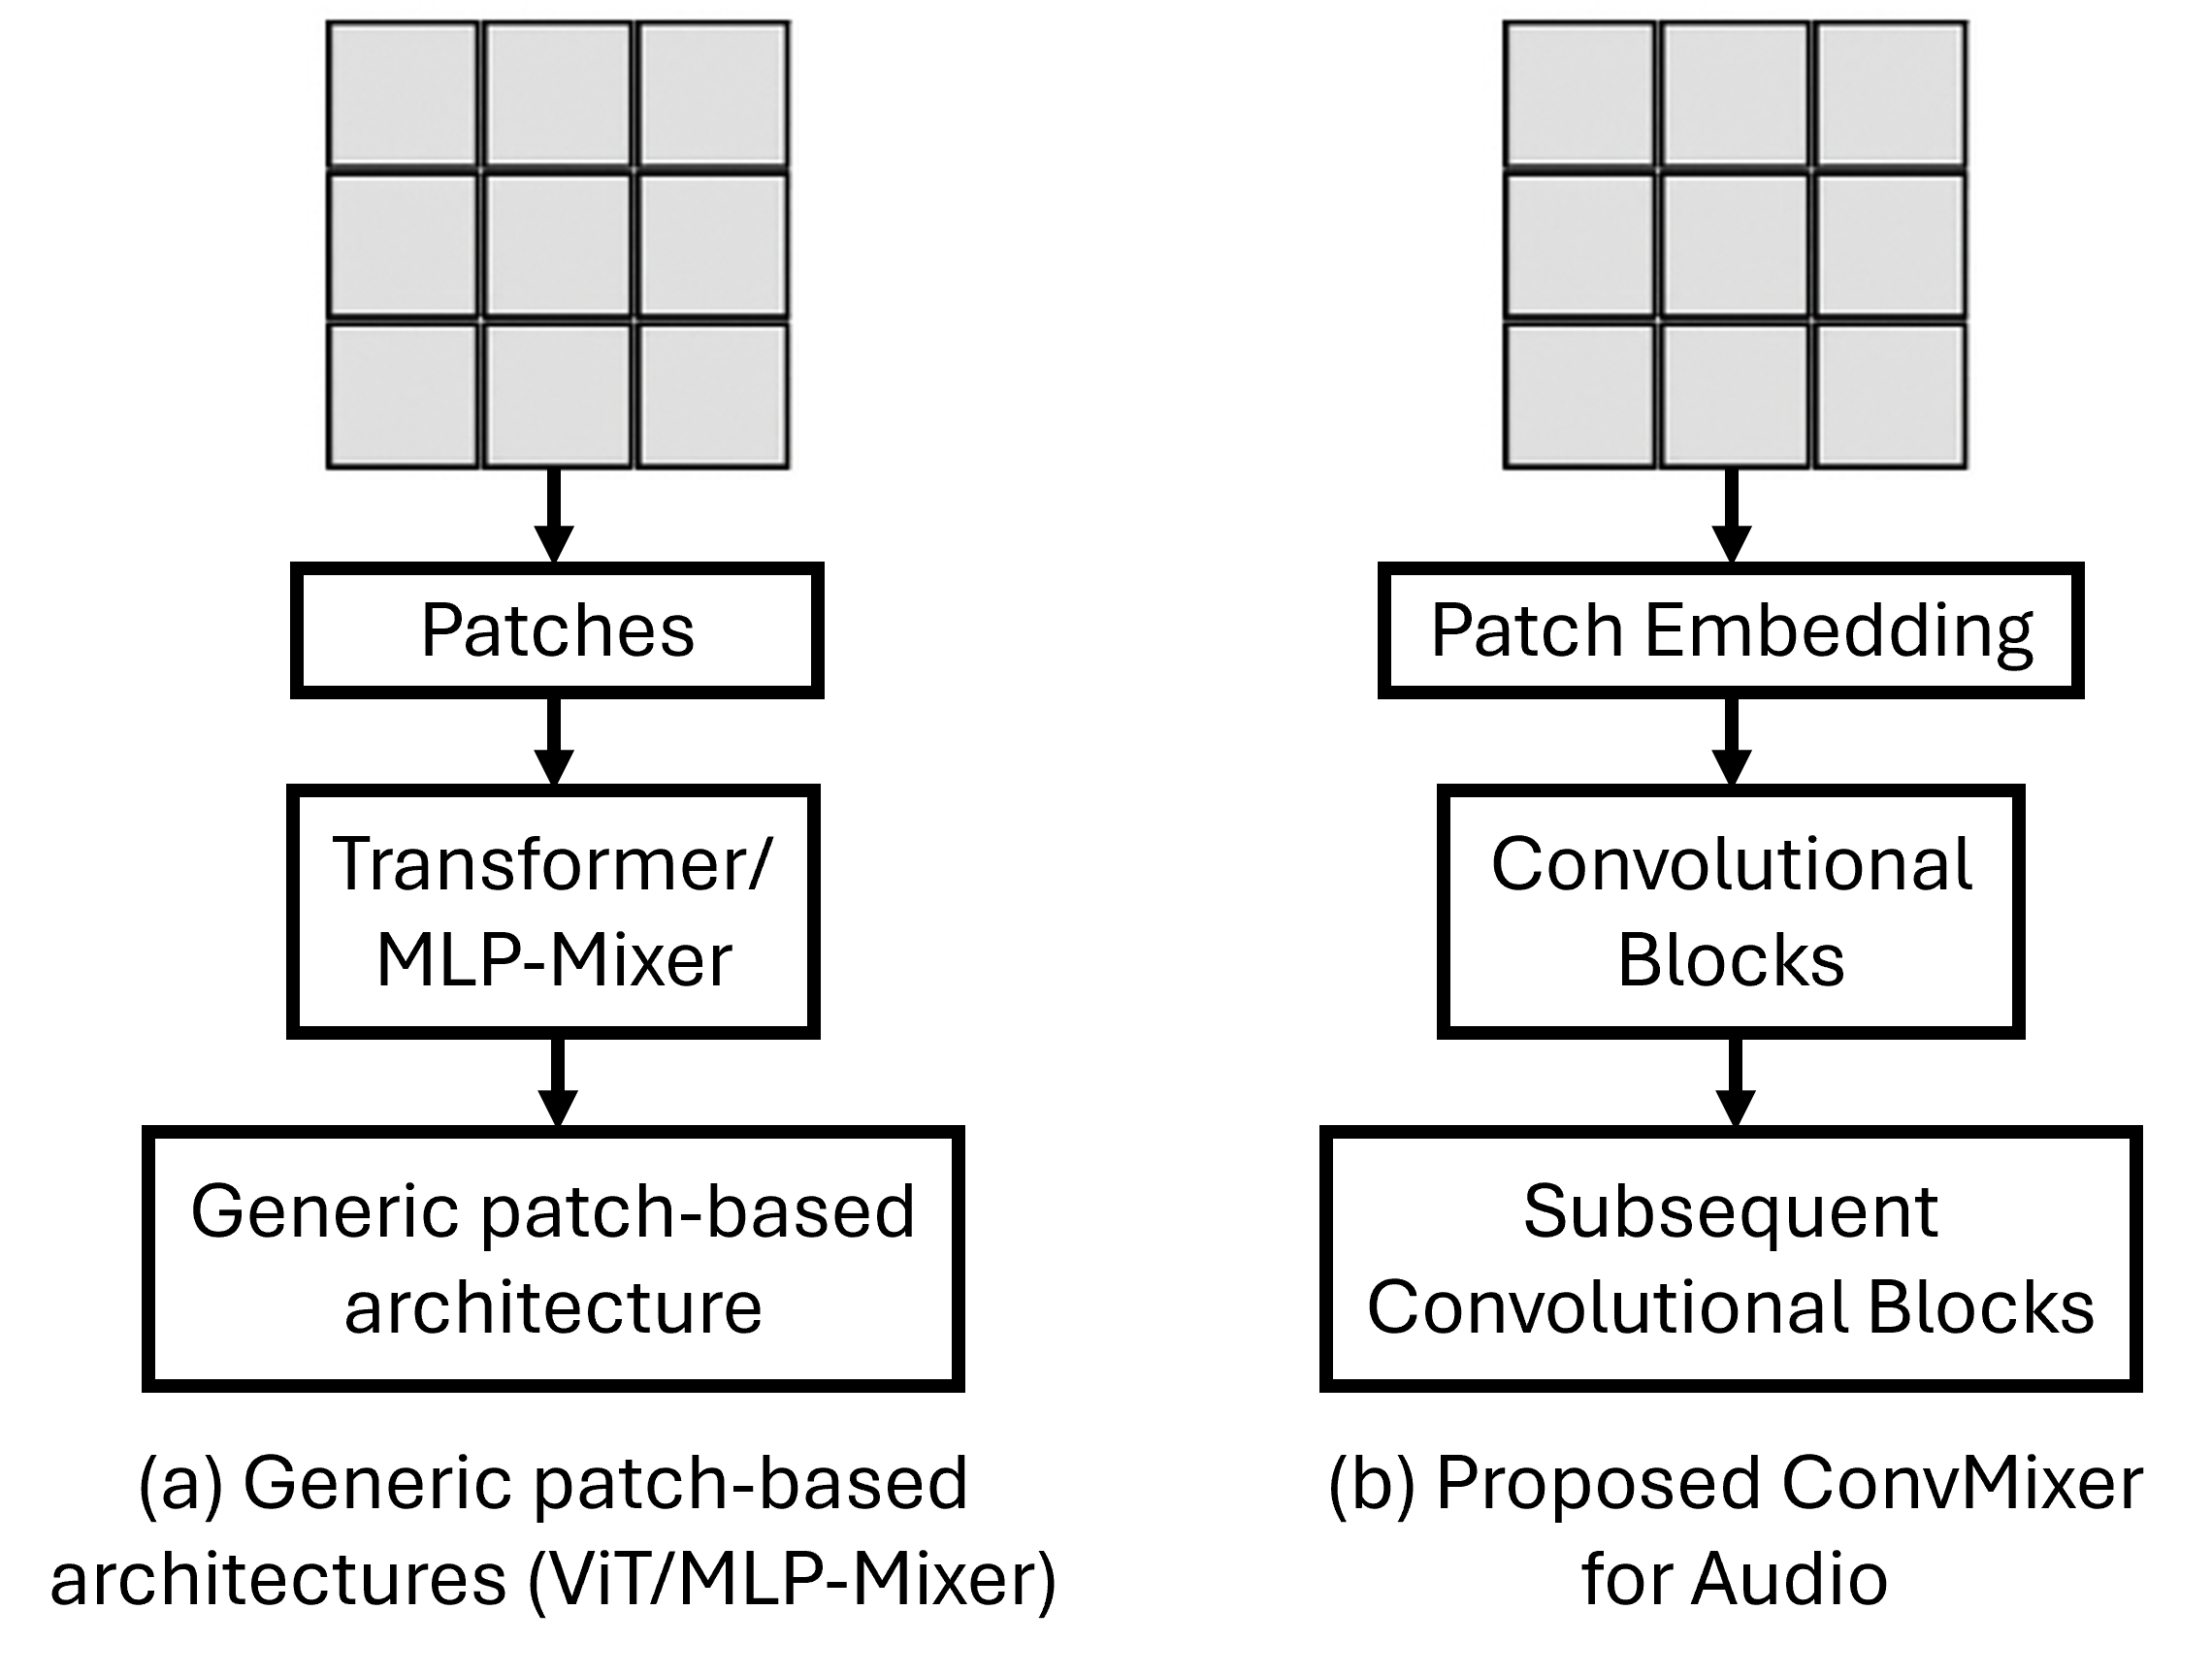
\includegraphics[width=0.55\linewidth]{imgs/Convmixer-comparison.png}
\caption{\label{fig:comparison}Conceptual comparison diagram of audio patch-based models.}
\end{figure}

The structure of this paper is organized as follows: Section 2 reviews related works, focusing on the evolution from CNNs to Transformer architectures and ConvMixer.
Section 3 details the proposed methodology, encompassing data preprocessing steps, Mel-spectrogram feature extraction, and the ConvMixer architecture.
Section 4 presents the experiments, quantitative results, and performance analysis.
Section 5 discusses the key findings, compares the model against foundational architectures, and addresses the study's limitations.
Finally, Section 6 provides the conclusion and outlines directions for future work.
